\documentclass{article}
	\usepackage[total={17cm,20cm},top=2cm, left=2cm]{geometry}
	%Paquetes adicionales
	\usepackage{latexsym,amsmath,amssymb,amsfonts}
	\usepackage[latin1]{inputenc}
	\usepackage[T1]{fontenc}
	\usepackage{graphicx}
	\graphicspath{ {/home/alejandro/Documentos/Examen} }
	\usepackage[spanish]{babel}
	\setlength{\parindent}{0cm}
	\pagestyle{empty}
	%------------Comandos especiales-------------------
	\newcommand{\R}{\mathbb{R}}
 	\newcommand{\Z}{\mathbb{Z}}
  	\newcommand{\Q}{\mathbb{Q}}
  	\newcommand{\C}{\mathbb{C}}
  	\newcommand{\N}{\mathbb{N}}
 	\newcommand{\I}{\mathbb{I}}
 	\newcommand{\F}{\mathbb{F}}
  	%-----------------------------------------------------------------
 
\begin{document}
{\sc CEIP REINA INVENTADA} \hfill Tiempo 0:45 minutos\\
{\sc $6^{\circ}$ ED Primaria Franc\'es} \hfill Puntuaje: 10 puntos\\
{\sc Evaluaci\'on Inicial}\\

{\bf Nom:}  \rule{40mm}{0.1mm} 
{\bf Pr\'enom:} \rule{60mm}{0.1mm}
{\bf Date:} \rule{30mm}{0.1mm}\\

{\bf Instrucciones.} Este es un examen de prueba inicial, trabaje de manera clara y ordenada. Buena suerte.\\

\begin{enumerate}
\item{\bf [1 Punto]} Comment tu t' apelles? \rule{107mm}{0.1mm}\\
\item{\bf [1 Punto]} Escribe los siguientes n\'umeros en Franc\'es:\\\\
	{\bf 20:}  \rule{47mm}{0.1mm} 
	{\bf 31:} \rule{47mm}{0.1mm}
	{\bf 43:} \rule{46mm}{0.1mm}\\\\
	{\bf 50:}  \rule{47mm}{0.1mm} 
	{\bf 16:} \rule{47mm}{0.1mm}
	{\bf 18:} \rule{46mm}{0.1mm}\\
\item{\bf [2 Puntos]} Escribe los d\'ias de la semana en Franc\'es: \rule{77mm}{0.1mm}\\\\
\rule{161mm}{0.1mm}\\
\item{\bf [2 Puntos]} Escribe los meses del a\~{n}o en Franc\'es: \rule{83mm}{0.1mm}\\\\
\rule{161mm}{0.1mm}
\item{\bf [1 Puntos]} Escriba los colores de la bandera francesa en Franc\'es y color\'eala:\\\\
\rule{161mm}{0.01mm}
\begin{figure}[h]
\begin{center}

\includegraphics[scale=0.05]{images.png}
\end{center}
\end{figure}
\item{\bf [1 Puntos]} ?`Cu\'al de las siluetas corresponde a Francia?\\
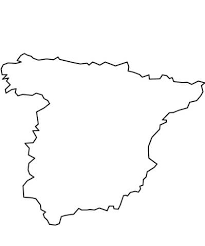
\includegraphics[scale=0.2]{images2.png}
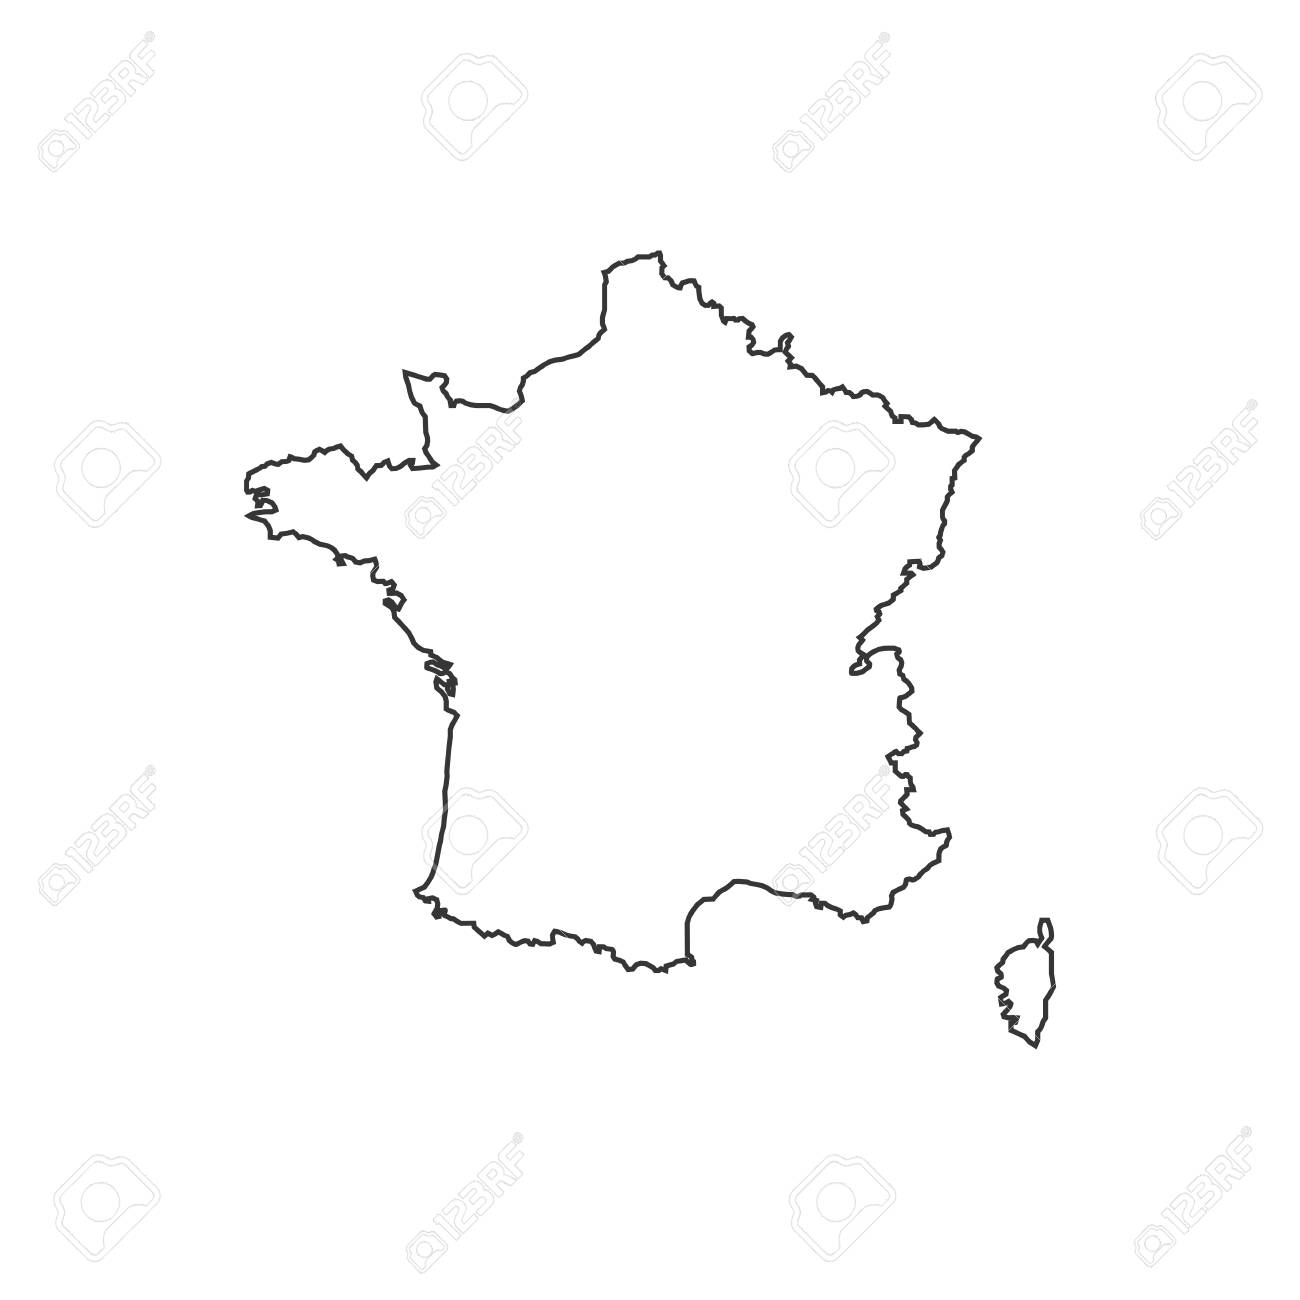
\includegraphics[scale=0.2]{images3.jpg}
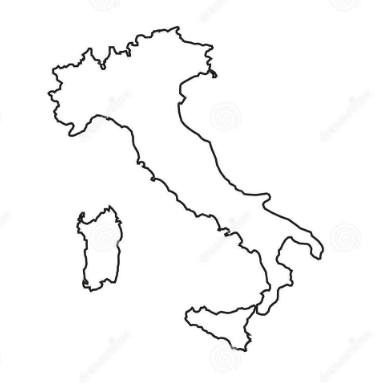
\includegraphics[scale=0.15]{images4.png}
\item{\bf [1 Puntos]} ?`Cu\'al es la capital de Francia? \rule{94mm}{0.1mm}\\
\item{\bf [1 Puntos]} Escriba dos monumentos importantes de Francia: \rule{68mm}{0.1mm}
\end{enumerate}
\end{document}